\documentclass[a4paper,12pt]{article}
\usepackage{polski}
\usepackage[utf8]{inputenc}
\usepackage[left = 3cm, right = 3cm, top = 2cm, bottom = 2cm]{geometry}
\usepackage{enumerate}
\usepackage{amssymb}		% pakiet do symboli
\usepackage{amsmath}		% pakiet do matmy
\usepackage{enumitem}		% punktowanie (a), (b), ...
\usepackage{nopageno}		% brak numerow stron
\usepackage{graphicx}		% wstawianie obrazkow
\usepackage{float}			% wstawianie obrazkow w dowolnym miejscu
\usepackage{titling}
\usepackage[]{algorithm2e} 	% algorytmy :))
\usepackage{program}

% nowe komendy dla wygodniejszego pisania :)
\newcommand{\subtitle}[1]{ \posttitle{ \par\end{center} \begin{center}\large#1\end{center} \vskip0.5em}}
\newcommand{\floor}[1]{\left\lfloor #1 \right\rfloor}
\newcommand{\ceil}[1]{\left\lceil #1 \right\rceil}

\begin{document}
\noindent \textbf{Lista 2, zadanie 9 - Tomasz Woszczyński}\newline

\noindent \newline \textbf{Treść:} Dla ważonego drzewa $T = (V, E; c)$, gdzie $c: V \to \mathbb{R}_{+}$, określamy jego zewnętrzną długość $EL(T)$ jako
$$ EL(T)= \sum\limits_{v-\text{liść}\in T}^{} c(v) \cdot d(v), $$ 
gdzie $d(v)$ jest długością ścieżki od korzenia do liścia $v$ (mierzoną liczbą krawędzi na ścieżce). Rozważmy następujący problem. Dany jest $n$-elementowy zbiór $\{ w_1, \dots, w_n \}$ dodatnich liczb rzeczywistych. Zadaniem jest znalezienie ważonego drzewa binarnego $T$ o $n$ liściach, takiego, że każda liczba $w_i$ jest wagą dokładnie jednego liścia oraz $T$ ma minimalną wagę $EL(T)$ pośród wszystkich drzew o tej własności. \newline

\noindent \textbf{Informacje:}  Mamy dane  $\{ w_1, \dots, w_n \}$ i wiemy, że $\forall i: w_i \in \mathbb{R}_{+}$, $c(v)$ jest wagą liścia $v$, a $d(v)$ długością ścieżki od korzenia do liścia $v$. Niech $Q$ będzie kolejką priorytetową z wagami, dla każdego wierzchołka możemy stworzyć pewnego rodzaju strukturę postaci $v(w_i, \text{NULL}, \text{NULL})$, gdzie $w_i$ jest wagą wierzchołka, a dwie ostatnie wartości (tj. NULL) są odpowiednio lewym i prawym poddrzewem wierzchołka $v$. Disclaimer do $Q.pop()$: bierzemy wartość pierwszego elementu, przypisujemy go do zmiennej $l$ lub $r$, a następnie usuwamy pierwszy element w $Q$.\newline

\noindent \textbf{Algorytm:} \newline
\begin{algorithm}[H]
	Wrzuć do $Q$ wagi liści\;  
	\While{$\vert Q \vert > 1$}{
		$l := Q.pop()$\;
		$p := Q.pop()$\;
		$Q.push(l.w + p.w, l, p)$\;
	}
	\Return $Q.pop()$\;
\end{algorithm} 

~\\ \noindent \textbf{Przykład:} Weźmy liście o wagach $\{ 5, 7, 2, 10, 8, 20, 30\}$. Wtedy kolejka przed wejściem w pętle $Q = \{ 2, 5, 7, 8, 10, 20, 30 \}$. Po pierwszym przejściu pętli będziemy mieć $Q = \{ 7, 7, 8, 10, 20, 30 \}$, po drugim $Q = \{8, 10, 14, 20, 30 \}$, po trzecim $Q = \{ 14, 18, 20, 30 \}$, aż w kolejce zostanie jeden element (korzeń drzewa), który umieścimy na samym końcu w procesie budowania drzewa. Poniżej rysunek przedstawia uzyskane drzewo $T$ (budujemy je od dołu).

\begin{figure}[H]
\centering
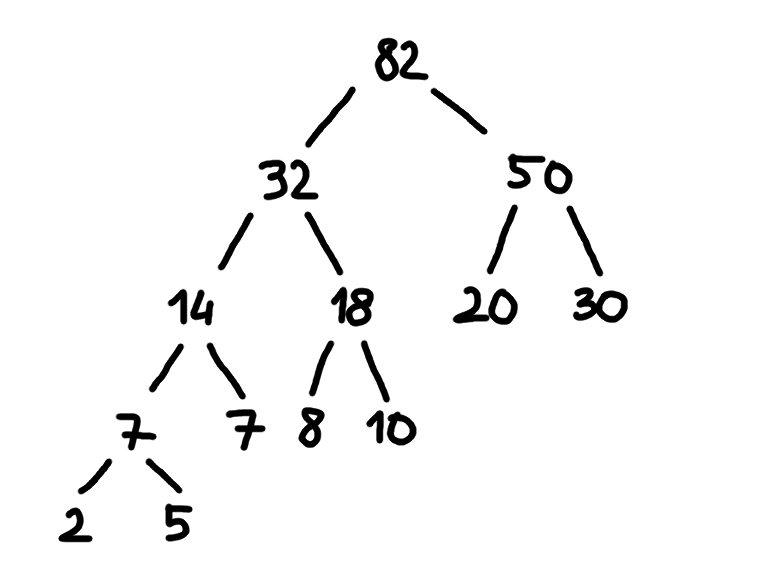
\includegraphics[width=0.5\textwidth]{drzewko.png}
\end{figure}

\noindent \textbf{Złożoność czasowa:} Algorytm działa w czasie $O(n log n)$, jako że pętla działa w czasie $O(n)$, a wstawienie elementu do kolejki prioretytowej w czasie $O(log n)$. Mnożąc te dwie wartości (jako że wstawienie elementu odbywa się w każdej iteracji pętli) daje nam wcześniej wspomnianą złożoność $O(n log n)$.  

~\\ \noindent \textbf{Dowód znajdowania minimalnego drzewa:} Niech $T$ będzie pełnym drzewem binarnym, oznaczmy jego zewnętrzną długość jako $EL(T)$, zbiór jego liści jako $L(T)$ oraz weźmy dwa wierzchołki $u, v$ o najmniejszych wagach. Możemy wtedy skonstruować drzewo $T'$ takie, że:
\begin{itemize}
\item jego zbiór liści to $L(T') = L(T) - \{ u, v\} \cup \{ w \}$, gdzie $w$ to nowo powstały wierzchołek poprzez połączenie dwóch o najmniejszych wagach,
\item $w(w) = w(u) + w(v)$,
\item $EL(T') \leq EL(T) - w(u) - w(v)$ oraz $EL(T') = EL(T) - w(u) - w(v)$, gdy $u$ i $v$ są rodzeństwem.
\end{itemize}
\noindent Podważmy istnienie drzewa $T'$. Gdy wierzchołki $u$ oraz $v$ są sąsiadami, możemy w prosty sposób stworzyć drzewo $T'$ z $T$ poprzez usunięcie $u$ oraz $v$ i dodanie $w$, czyli nowego liścia będącego ich rodzicem. Wtedy 
$$
\begin{aligned}
EL(T') &= EL(T) - w(u) \cdot d(u) - w(v) \cdot d(v) + w(w) \cdot d(w) = \\
          &= EL(T) - w(u) \cdot x - w(v) \cdot x + w(w) \cdot (x - 1) = \\
          &= EL(T) - w(u) - w(v)
\end{aligned}
$$
\noindent zakładając, że $x = d(u) = d(v) = d(w) + 1$, a więc długości ścieżek od korzenia do $u$ oraz do $v$ są równe. \newline
W przeciwnym wypadku załóżmy bez straty ogólności, że $d(u) \geq d(v)$ i niech $r$ będzie rodzeństwem $u$, który niekoniecznie jest liściem. Zamieniamy wtedy miejscami $v$ z $r$, a wiedząc że $d(r)$ jest co najmniej tak długa jak ścieżka z $u$, to zewnętrzna długość $EL(T)$ może tylko zmaleć. Wtedy wykonujemy kroki opisane powyżej.

~\\ \noindent \textbf{Dowód znajdowania optymalnego wyniku:} Załóżmy, że drzewo $T$ uzyskujemy poprzez działanie naszego algorytmu i weźmy inne drzewo $U$, dla którego zbiory liści i wag są równe tym zbiorom drzewa $T$. Wtedy $EL(T) \leq EL(U)$. Udowodnimy ten lemat indukcyjnie. Dla dwóch liści w drzewie jest to oczywiste, gdyż zachodzi równość. W przeciwnym wypadku mamy do czynienia z większą ilością liści w drzewie, wybierzmy więc liście $u$ oraz $v$ wybrane przez algorytm. Konstruujemy wtedy drzewa $T'$ oraz $U'$, takie że
\begin{itemize}
\item $EL(T') = EL(T) - w(u) - w(v)$,
\item $EL(U') \leq EL(U) - w(u) - w(v)$.
\end{itemize}
\noindent $T'$ jest drzewem tworzonym przez algorytm, załóżmy że ma on $n-1$ liści, wtedy możemy skorzystać z założenia indukcyjnego, dzięki czemu otrzymamy $EL(T') \leq EL(U')$, a więc ostatecznie mamy
$$
\begin{aligned}
EL(T) &= EL(T') + w(u) + w(v) \leq \\
         &\leq EL(U') + w(u) + w(v) \leq \\
         &\leq EL(U)
\end{aligned}
$$
co kończy dowód. $\blacksquare$

\end{document}